

%%%%%%%%%%
\begin{figure}
\centering
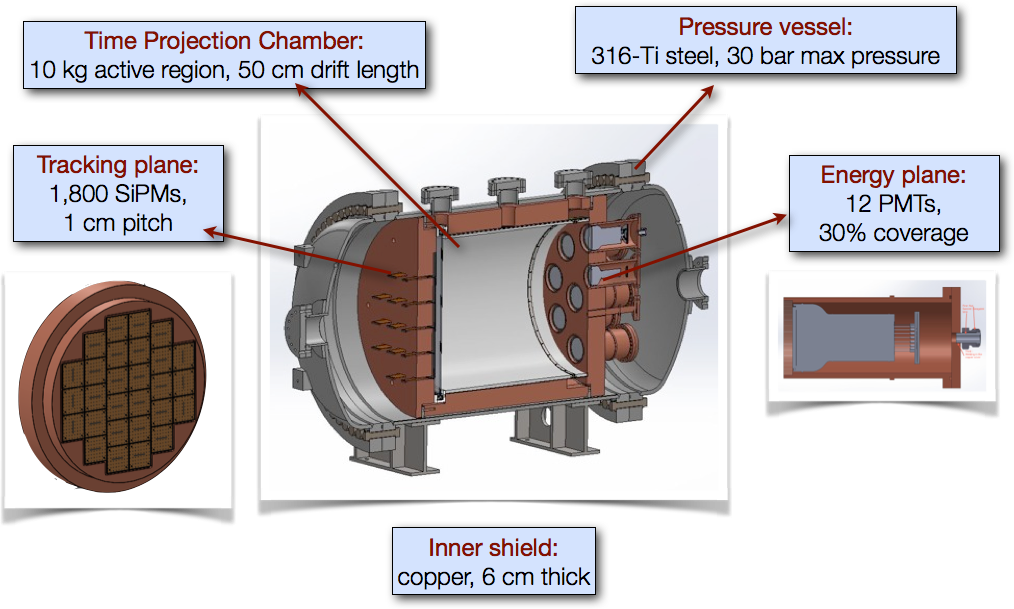
\includegraphics[width=0.9\textwidth]{img2/NEW.png}
\caption{\small The NEW apparatus.} \label{fig:NEW}
\end{figure} 

%%%%%%%%%%
\begin{figure}
\centering
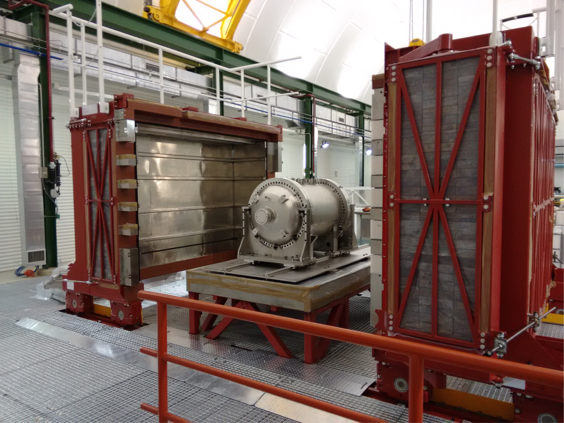
\includegraphics[width=0.9\textwidth]{img2/NewCastle.png}
\caption{\small The NEW detector, sitting inside the Lead Castle at the Canfranc Underground Laboratory.} \label{fig.NewCastle}
\end{figure} 

%\begin{figure}
%\centering
%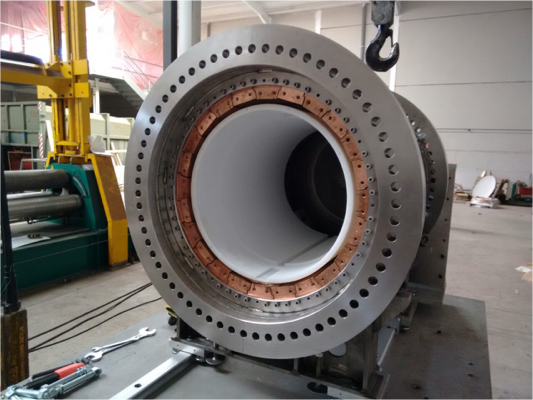
\includegraphics[width=0.9\textwidth]{img2/NewICS.png}
%\caption{\small The NEW detector, showing the inner copper shield (ICS), 6 cm thick and the outer frame of the field cage.} \label{fig.NewICS}
%\end{figure} 

\begin{figure}
\centering
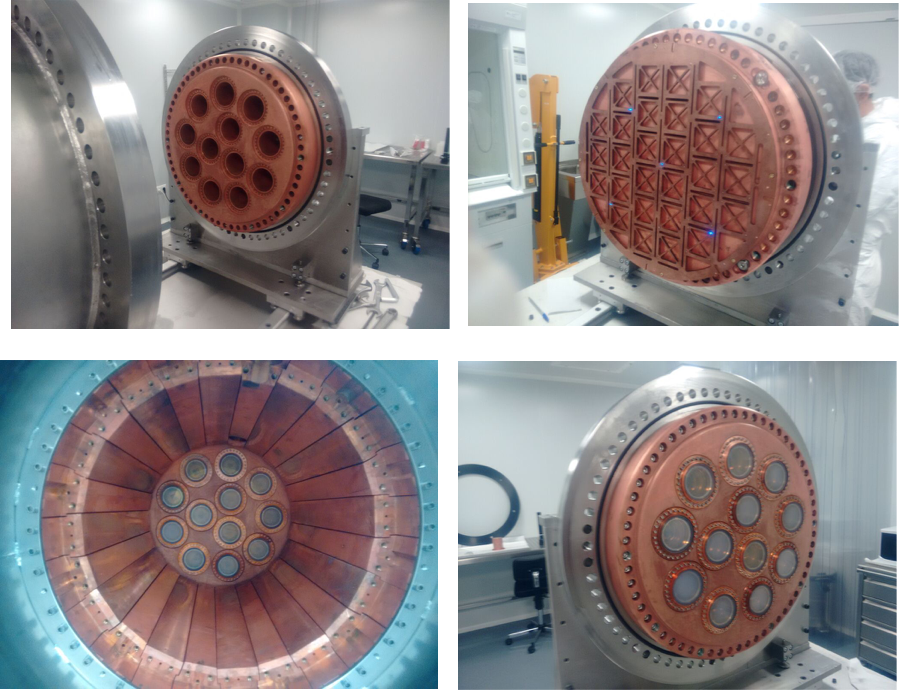
\includegraphics[width=0.9\textwidth]{img2/EP.png}
\caption{\small Top left: energy plane support; top right: tracking place
support; bottom left: energy plane installed inside NEW, with the PMTs in place; 
top right; energy plane displaying the sapphire windows, coated with TPB.} \label{fig.EP}
\end{figure} 


\begin{figure}
\centering
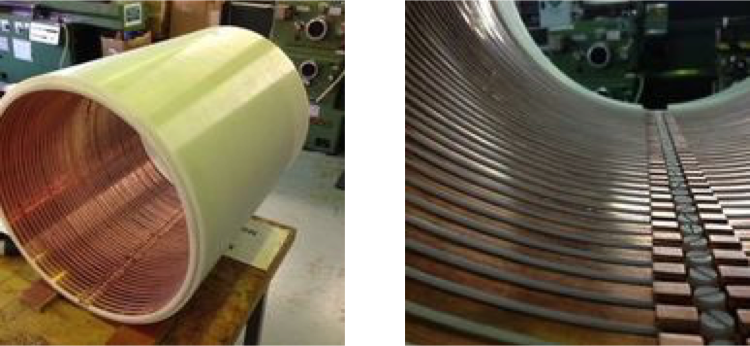
\includegraphics[width=0.9\textwidth]{img2/FieldCage.png}
\caption{\small The NEW field cage mounts copper rings connected by radiopure resistors in a cylindrical body of high density polyethylene. The field cage has 0.5 m diameter and 0.5 m length.} \label{fig.FC}
\end{figure}


The NEW (NEXT-WHITE) apparatus\footnote{The name honours the memory of the late Professor James White, one of the key scientists of the NEXT Collaboration.}, shown in Figure \ref{fig:NEW}, is the first phase of the NEXT detector to operate underground (Figure \ref{fig.NewCastle}). NEW 
is a scale 1:2 in size (1:8 in mass) of NEXT-100. The energy plane contains 12 PMTs (20 \% of the 60 PMTs deployed in NEXT-100, see Figure \ref{fig.EP}). The tracking plane technology consists of 30 Kapton Dice Boards (KDB) deploying 1800 SiPMs (also 20\% of the sensors). The field cage has a diameter of 50~cm and a length of 50~cm (Figure \ref{fig.FC}). 

NEW is a major step for the NEXT project, and will allow us to address a number of crucial questions. Specifically:

\begin{enumerate}
\item {\bf Energy resolution}: the aspect ratio of NEW is the same to that of NEXT-100 (and DBDM, but better than DEMO). The larger dimensions of the detector allow to contain large tracks and therefore to include in the study energetic sources. This will permit a study of the resolution at 511 keV and 1.2 MeV (\NA\ source), 660 keV (\CS\ source), 1.5 MeV and 2.6 MeV (\THO\ source). 
\item {\bf Topological signature}: we will repeat the analysis that we have just carried out in DEMO, using 511 keV, 660 keV, 1.2 MeV and 2.6 MeV single electrons (from \NA, \CS\ and \THO\ sources) as well as double electrons from the \TL\ double escape peak to understand with detail the efficiency and rejection power of the topological signature. 
\item {\bf Background model:} Comparison of data and Monte Carlo should help us to validate our background model (currently based exclusively in Monte Carlo calculations) and to identify and correct possible hot spots.
 \item {\bf Impact of radon:} In 2016 NEW will operate inside a radon-free tent (the infrastructure has been approved by the LSC and in currently being ordered to the vendor). Analysis of our data and Monte Carlo comparison should permit the quantification of the effect of radon degassing inside the detector.
 \end{enumerate}

In addition, NEW will allow us to quantify any potential technical issues. Among these:
 
 \begin{enumerate}
\item {\bf S1 and S2 signals}: We will measure the number of photoelectrons for S1 and S2 signals produced near \Qbb\, in order to ensure that photoelectron statistics does not degrade the energy resolution. The effect of sapphire windows and TPB coating in light collection will be evaluated (DEMO used bare PMTs sensitive to VUV and very radioactive).  
\item {\bf Electron lifetime}: DEMO achieved electron lifetimes in excess of 10 ms. The same or better should be achieved with NEW. A much better measurement can be made here, given the long drift in NEW field cage. 
\item {\bf Operational stability and sparks:} In DEMO the frequency of sparks was of the order of one a week. NEW uses a quartz plate coated with ITO in the region facing the SiPMs. Sparks should be rare, but its frequency and effect (e.g, in the TPB coating the plate) must be measured. 
 \item {\bf Leaks:} The energy plane is separated from the main volume defined by the field cage by a plate sealing the PMTs, which operate in vacuum. The PMTs are coupled to the main volume by sapphire windows. The system needs to operate without leaks between the main volume in the energy plane for long periods of time.
 \end{enumerate}

Other important issues where NEW will allow steady progress are:

 \begin{enumerate}
\item {\bf Gas system}, which is the same that will be used for NEW-100. In particular, NEW will test for more than one year the state-of-the-art, triple-metal-sealing compressor manufactured by the German company SERA for NEXT, before operation with enriched xenon. 
\item {\bf FEE, DAQ and SC}: The front-end electronics of the PMTs and SiPMs, the DAQ system and the slow controls are identical for NEW and NEXT-100, and operation of the former will allow to spot and correct any unforeseen issues. 
 \end{enumerate}
 
